\chapter{Conclusions}

This project explores the application of machine learning techniques to automate Fantasy Premier League and its potential use to maximise performance. With the use of historical data, predictive modelling, and optimisation algorithms this project aims to create a system capable of performing amongst the top players of FPL.

Long Short-Term Memory (LSTM) networks were selected for their ability to model temporal dependencies and will be tested with the expectation of outperforming traditional regression models when predicting player performance. A multi-stream approach was adopted to enhance system accuracy by tailoring predictions to specific player positions. Additionally, optimisation algorithms will be implemented to tackle team selection. Multiple selection strategies will be evaluated to identify the most effective approach, from statistical methods to strategies inspired by top-performing FPL managers.

The research shows the potential of machine learning on this topic, where predictive accuracy and adaptability can offer a competitive edge. While progress has been made in data preprocessing, model selection, and system implementation, challenges such as data integration and evaluation remain areas that need further development.

There are some limitations to this project that, while not critical, are worth mentioning. To properly evaluate the results, it will be necessary to run multiple simulations across different seasons and configurations, each with significant data requirements. This might require significant computational power, but the High-Performance Computing services at The University of Sheffield could help address this. Additionally, predicting the performance of new and young players presents a big challenge due to the lack of publicly available data. Multiple data sources will ideally be used to address this, but this approach carries risks. Ensuring the integrity of the data will require careful validation throughout the project.

This project establishes a solid foundation for FPL automation. By refining the predictive models and optimisation strategies, the system holds the potential to rival top-performing users. Figure~\ref{fig:gantt_chart} presents an overview of the general plan for the remaining time of the project, highlighting key deadlines.

\begin{figure}[H]
    \centering
    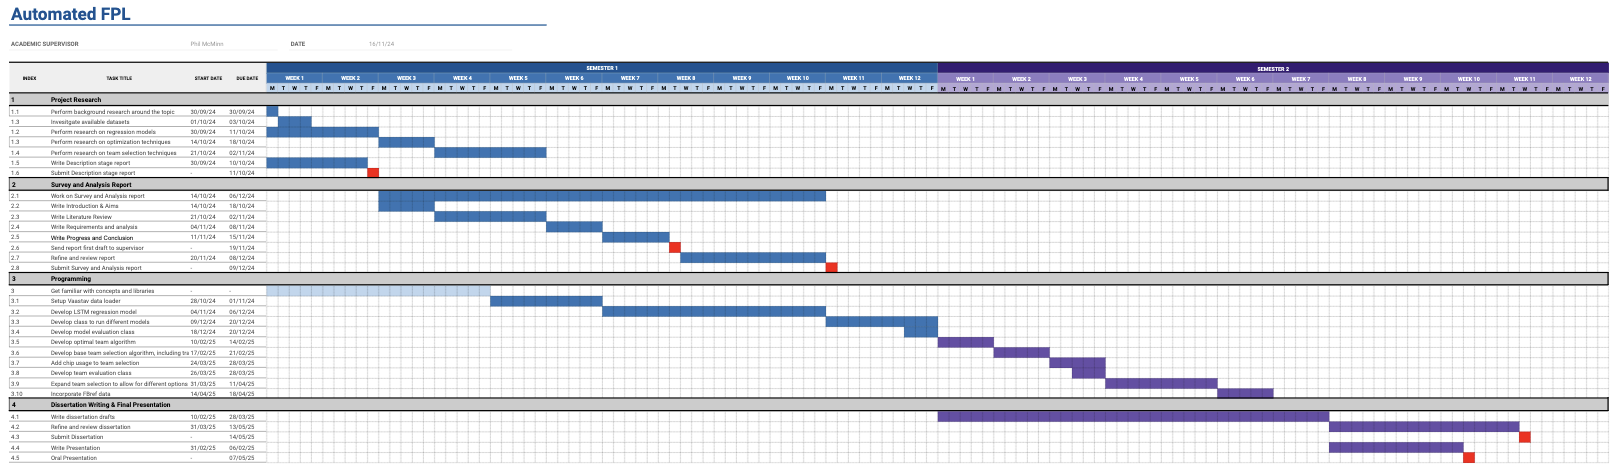
\includegraphics[width=15cm]{images/gant_chart.png}
    \caption{Overview of the project timeline}
    \label{fig:gantt_chart}
\end{figure}

Figure \ref{fig:gantt_chart} lays out a clear step-by-step breakdown of how each stage of the project will be tackled. There’s some uncertainty about how long it will take to implement the LSTM model, so extra time has been accommodated in case of any unexpected delays. Similarly, the expansion of team selection techniques has been planned for later in the project, with additional time allocated due to the unpredictability of how much time will be available to explore a wide range of methods. Finally, incorporating FBref data is considered a nice-to-have rather than a core part of the project and its inclusion will depend on how much time remains in the final stages.
